\section{Durchführung}
\label{sec:Durchführung}
Im gesamten Versuch wird der Aufbau in Abb. \ref{fig:aufbau} verwendet.
\newline
Vor Beginn muss der Strahl justiert werden. Dazu werden die beiden hellsten
Punkte durch Verstellen eines Spiegels übereinander auf den Eintrittsspalt des 
Photoelements gelegt.

\begin{figure}
    \centering
    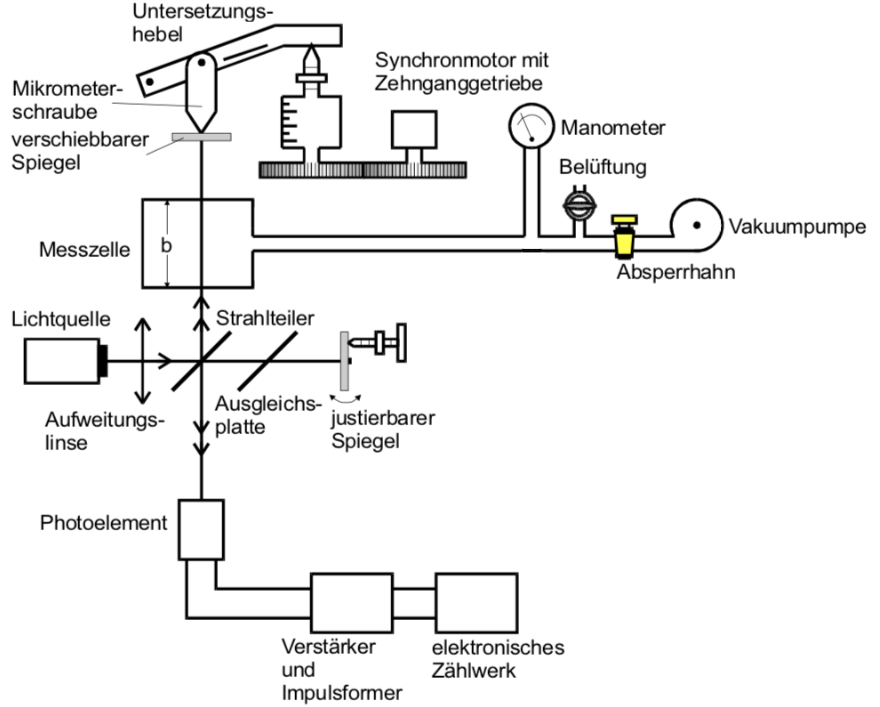
\includegraphics[width=12cm, height=10cm]{build/aufbau.png}
    \caption{Es ist der Aufbau des Michelson-Interferometers zu sehen.
    Außerdem ist ein Teil zur Zählung der Impulse und eine Vakuumpumpe
    hinzugefügt. \cite{V401}}
    \label{fig:aufbau}
\end{figure}

\subsection{Messung der Wellenlänge}
Mithilfe des Michelson-Interferometers wird die Wellänge eines Lasers bestimmt.
Einer der Spiegel wird durch eine Mikrometerschraube mithilfe eines Motors in 
Strahlrichtung verschoben. Dabei werden die Maxima durch ein Photoelement gezählt.
Der Spiegel wird so lange verschoben, bis mindestens $\num{3000}$ Maxima registriert
sind. Die Abstandsdifferenz des Spiegels wird aufgenommen. Das Ganze wird $\num{10}$ mal durchgeführt.

\subsection{Messung des Brechungsindex}
Der Brechungsindex von Luft wird gemessen, indem durch eine Vakuumpumpe der Innendruck
auf $\SI{0.4}{\bar}$ erniedrigt wird. Anschließend wird durch ein Ventil Luft
reingelassen und die Maxima, die registriert werden, bis der Innendruck wieder auf
$\SI{1}{\bar}$ gestiegen ist, werden gezählt. Der Vorgang wird $\num{10}$ mal durchgeführt.